\subsection{Newton with Adaptive Bisection Starts (Newton-ABS)}\label{ssec:newton-abs}

In this section, we improve Newton's Method described in~\Cref{ssec:newton}.
Specifically, we first discuss how to find lower and upper bounds $h_\star$, $h^\star \in [0,\infty)$,
respectively, such that the root lies in $[h_\star, h^\star]$.
We then discuss an adaptive bisection method that preceeds Newton's Method
to find a clever initial point $h^{(0)}$.

We first begin with the discussion of $h_\star$ and $h^\star$.
Note that the root-finding problem for $\varphi$
is equivalent to finding the largest value $h > 0$ such that $\varphi(h) \geq 0$, or
\begin{align}
    \sup\set{
        h > 0 :
        \sum\limits_{i=1}^p
        \frac{v_i^2}{(\Sigma_{ii} h + \lambda)^2}
        \geq
        1
    }
    \label{eq:newton-abs:lower-bound-problem}
\end{align}
In~\Cref{appendix:newton-abs:bounds}, we show that we can relax this problem
and solve an approximate problem using Cauchy-Schwarz
to get $h_\star$ such that $\varphi(h_\star) \geq 0$.
Similarly, to derive $h^\star$, we begin with the problem of finding the smallest $h$ such that
$\varphi(h) \leq 0$, or
\begin{align}
    \inf\set{
        h > 0
        :
        \sum\limits_{i=1}^p
        \frac{v_i^2}{(\Sigma_{ii} h + \lambda)^2}
        \leq
        1
    }
    \label{eq:newton-abs:upper-bound-problem}
\end{align}
\Cref{appendix:newton-abs:bounds} also shows that through a different approximation,
we can derive $h^\star$ such that $\varphi(h^\star) \leq 0$.
This shows that the root must lie in $[h_\star, h^\star]$.

In practice, $\varphi$ may decay incredibly rapidly near $h \approx 0$ and have an extremely flat tail
(see~\Cref{fig:newton-abs:stuck}).
To protect against slow convergence of Newton's Method in this case,
we may use $h_\star$ and $h^\star$ to first perform a bisection method to find the initial starting point.
The key idea is to use bisection first for a few iterations 
to avoid the region of fast decay before applying Newton's Method.
Once bisection gives a sufficiently close value to the root, 
we apply Newton's Method for fast, guaranteed convergence.
Although one may use \emph{any} bisection method to split the interval $[h_\star, h^\star]$,
e.g. the simple bisection that splits the interval in halves,
we propose an \emph{adaptive bisection method} that has been most effective.

We now describe our proposed adaptive bisection method.
Ideally, we would like to know if the root is closer to $h_\star$ or $h^\star$.
If we believe that the root is much closer to $h_\star$,
we do not have to bisect $[h_\star, h^\star]$ at the mid-point, 
but perhaps at a point closer to $h_\star$.
Likewise, if the root were much closer to $h^\star$, 
we would like to bisect at a point closer to $h^\star$.
Since we do not know the root, we would like to quantify a \emph{prior} of 
the root being closer to $h_\star$.
With this in mind, we note that in the derivation of $h^\star$
in~\Cref{appendix:newton-abs:bounds}, we 
approximated the problem of finding the smallest $h$ such that $\varphi(h) \leq 0$
by solving the problem for an upper bound of $\varphi$ (see~(\ref{eq:nmab:upper-approx})).
Then, the more accurate the approximation, the closer the approximate solution $h^\star$ is to the root.
The approximation essentially came from using the trivial fact that $\Sigma_{ii} h^\star \leq \Sigma_{ii} h^\star + \lambda$.
This motivates us to consider the worst approximation error (rate)
\begin{align*}
    w
    := 
    \max\limits_{i: \Sigma_{ii} > 0} \frac{\lambda}{\Sigma_{ii} h^\star + \lambda}
    =
    \frac{\lambda}{\Sigma_\star h^\star + \lambda}
    \in 
    (0,1)
\end{align*}
where $\Sigma_\star := \min\limits_{i : \Sigma_{ii} > 0} \Sigma_{ii}$.
If $w$ is small, the approximation in~(\ref{eq:nmab:upper-approx}) is tight,
which implies that the root is close to $h^\star$.
Hence, $1-w$ represents the prior that the root is close to $h^\star$.
We bisect at the new point $h := wh_\star + (1-w)h^\star$.
If $\varphi(h) \geq 0$, we use $h^{(0)} := h$ as the initial point for Newton's Method.
Otherwise, we set $h^\star := h$ and repeat the argument.
\Cref{alg:nabs:ab} summarizes this procedure.
Combining \Cref{alg:nabs:ab} with Newton's method,
we have \Cref{alg:nabs:nabs},
which we call \emph{Newton with Adaptive Bisection Starts} (Newton-ABS).

\begin{algorithm}[t]
    \caption{Adaptive Bisection}\label{alg:nabs:ab}
    \KwData{$\Sigma$, $v$, $\lambda$, $\varepsilon$}
    compute $h_\star$ that solves
    $
        \sum\limits_{i=1}^p
        (\Sigma_{ii} h + \lambda)^2
        \leq
        \norm{v}_1^2
    $ and take the positive part\;
    $
        h^\star
        \gets
        \sqrt{
            \sum\limits_{i: \Sigma_{ii} > 0} \frac{v_i^2}{\Sigma_{ii}^2}
        }
    $\;
    $\Sigma_\star \gets \min\limits_{i : \Sigma_{ii} > 0} \Sigma_{ii}$\;
    $w \gets \frac{\lambda}{\Sigma_\star h^\star + \lambda}$\;
    $h \gets wh_\star + (1-w)h^\star$\;
    \While{$\varphi(h) < 0$ and $\abs{\varphi(h)} > \varepsilon$}{
        $h^\star \gets h$\; 
        $w \gets \frac{\lambda}{\Sigma_\star h^\star + \lambda}$\;
        $h \gets wh_\star + (1-w)h^\star$\;
    }
    return $h$;
\end{algorithm}

\begin{algorithm}[t]
    \caption{Newton with Adaptive Bisection Starts (Newton-ABS)}\label{alg:nabs:nabs}
    \KwData{$\Sigma$, $v$, $\lambda$, $\varepsilon$}
    $h \gets$ result of \Cref{alg:nabs:ab}\;
    \If{$\abs{\varphi(h)} > \varepsilon$} {
        $h \gets$ result of Newton's Method starting at $h^{(0)} = h$\;
    }
    $\beta^\star \gets (\Sigma + \lambda h^{-1} I)^{-1} v$\;
    return $\beta^\star$\;
\end{algorithm}

Algorithm~\ref{alg:nabs:nabs} can be further optimized.
For example, if $h^\star - h_\star$ is below some threshold (e.g. $0.1$),
then we may skip bisection entirely and start Newton's Method at $h^{(0)} = h_\star$.
This is because the adaptive bisection may move too slowly if the range is too small.
From experimentation, this happens relatively often.
On a similar note, one may also enforce enough movement towards $h_\star$
by taking the max of $w$ with a minimal probability (e.g. $0.05$).
This will ensure that at least some proportion of $h_\star$ is taken 
if the prior is too strongly suggestive that the root is close to $h^\star$.
The idea is that it is always better to overshoot towards $h_\star$ such that $\varphi$ is non-negative,
so that Newton's Method can quickly converge down to the root,
than to slowly bisect to the root.

\Cref{fig:newton-abs:stuck} shows a plot of the Newton iterations for 
the vanilla Newton's Method from~\Cref{ssec:newton} and our proposed Newton-ABS.
It is clear from the right panel that Newton's Method struggles 
where there is a sharp decay near the origin, since the Newton iterations
slowly exit the kink.
However, Newton-ABS gets around this problem by moving from the upper bound $h^\star$
towards the origin until $\varphi$ is non-negative.
Hence, Newton-ABS first travels on the tail of $\varphi$ to find an initial point,
which is very likely to lie on the tail as well.

\begin{figure}[t]
    \centering 
    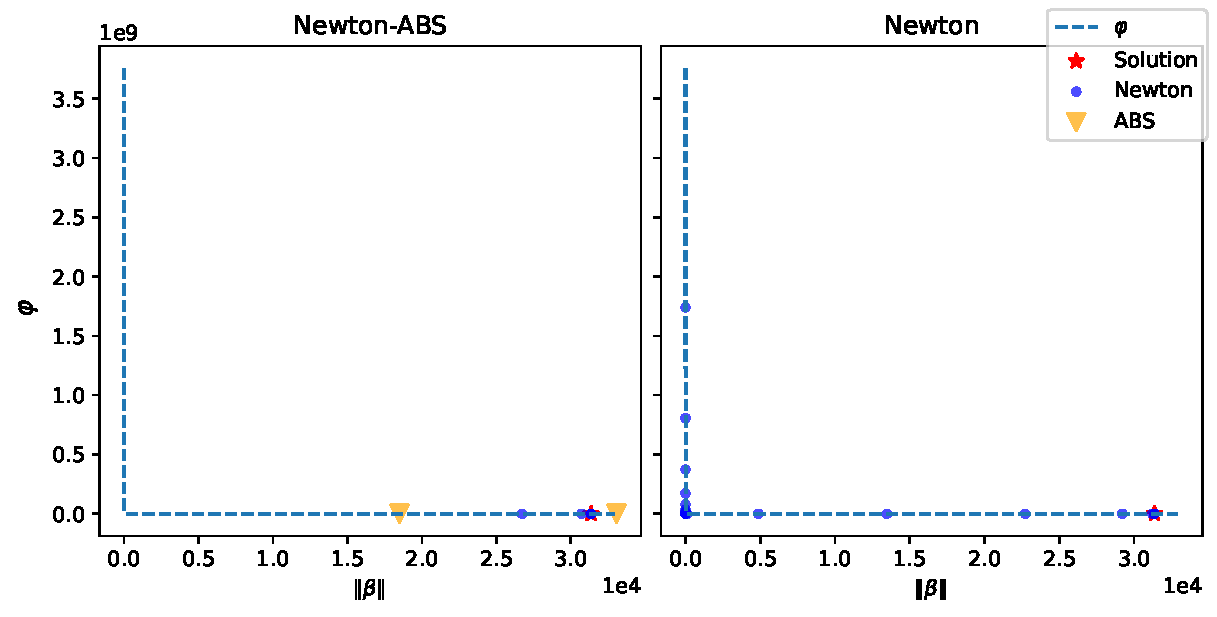
\includegraphics[width=0.7\textwidth]{figures/newton_stuck.pdf}
    \caption{Plot of Newton iterations for Newton's Method and Newton-ABS.
        It is clear from the right panel that Newton's Method struggles 
        when there is a sharp decay near the origin, since the Newton iterations
        slowly exit the kink.
        Newton-ABS goes around this problem by finding a good initial point
        sufficiently away from the origin.
    }
    \label{fig:newton-abs:stuck}
\end{figure}

\Cref{alg:nabs:nabs} is an effective way to leverage the power of both Newton Method and bisection.
Similarly, there are other methods such as Dekker's Method and Brent's Method
that combine many root-finding methods such as inverse quadratic interpolation,
secant method, and bisection method to leverage their different merits~\citep{brent:2013,dekker:1969}.
In~\Cref{fig:bench:newton-compare},
we also include benchmark results of Brent's Method
and find that Newton-ABS is superior. 
We refer to the full benchmark comparison to~\Cref{ssec:benchmark:pgd-newton}.
